\begin{figure*}[t]
\Fig[b]{.8\columnwidth}{%
\hspace{-.6em}%
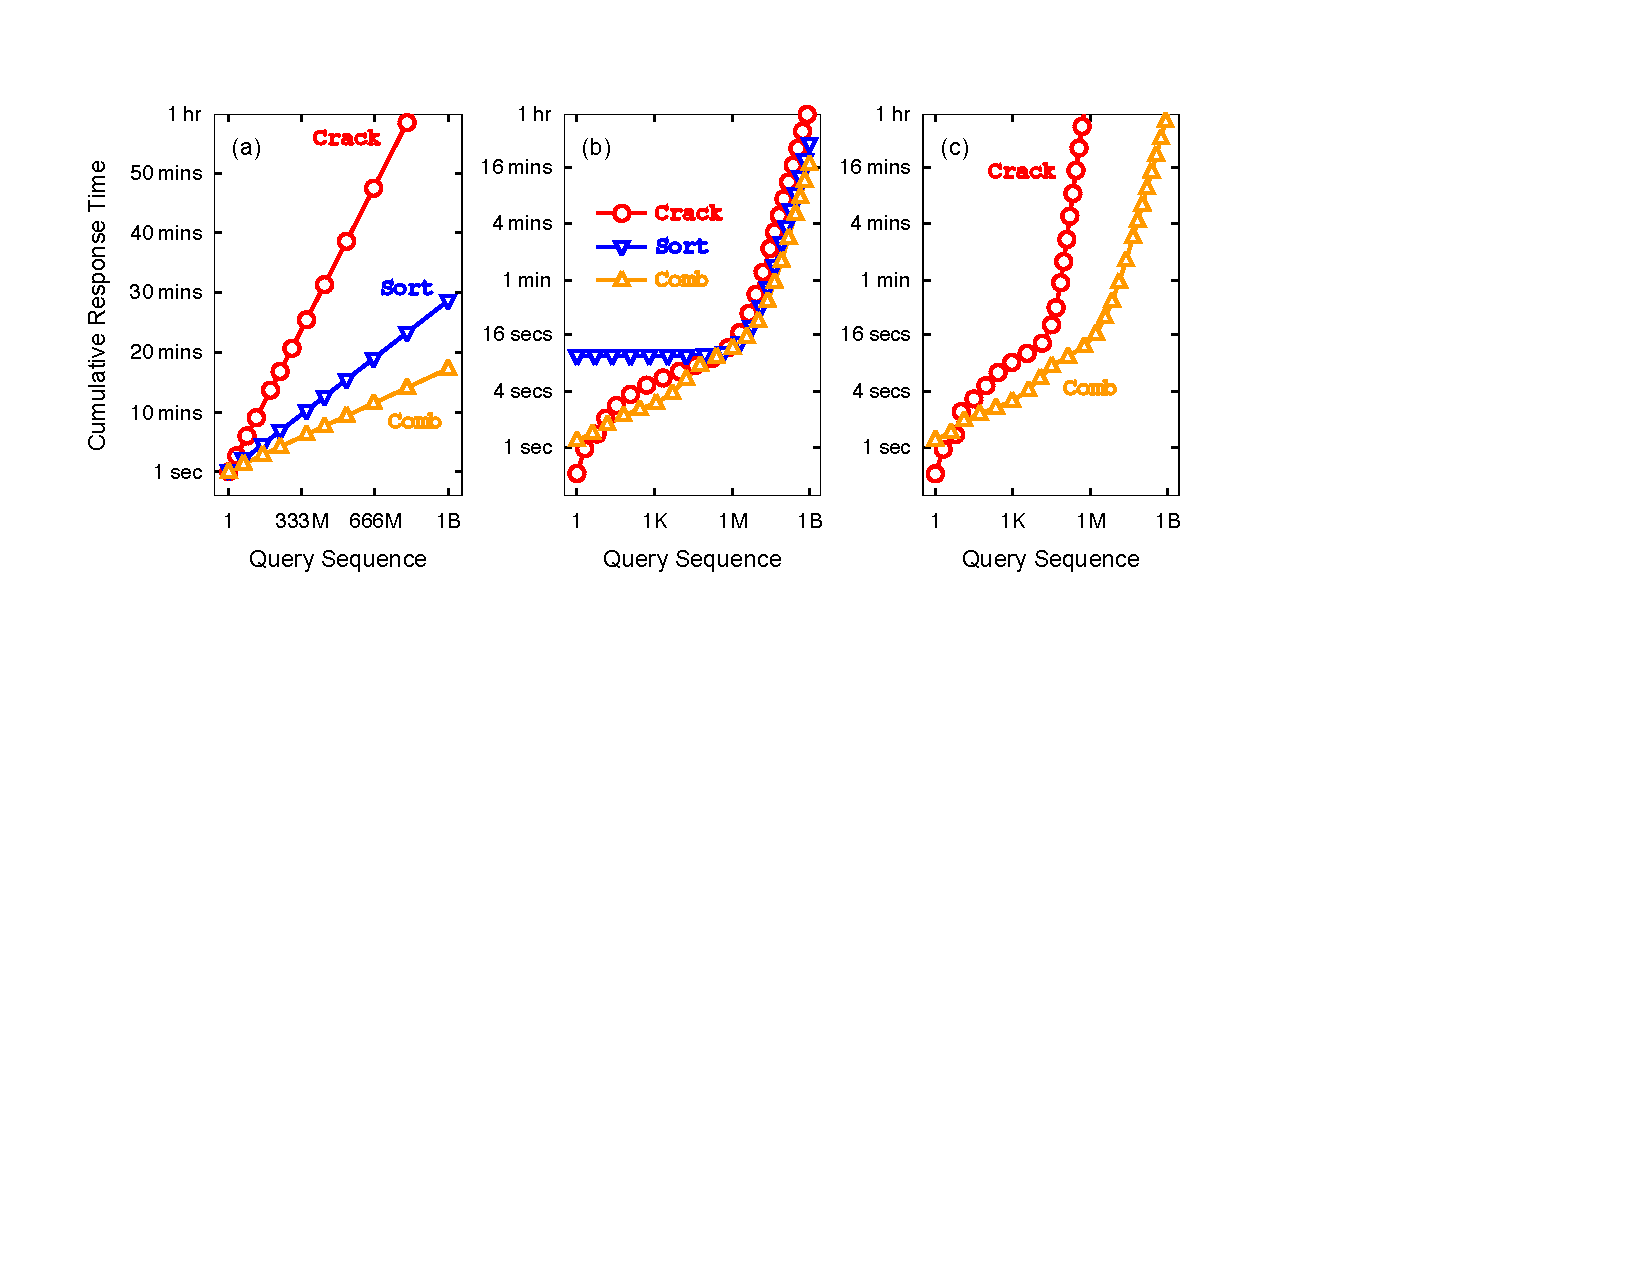
\includegraphics[width=1.35\columnwidth]{graphs/fig_basic_crake.pdf}%
\vspace{-1em}
\caption{Resilient adaptive indexing with Comb.}
\vspace{-1em}
\label{F:BasicPerQueryComb}
}
\hfill
\hspace{5.5em}%
\Fig[b]{.55\columnwidth}{%
\hspace{2em}%
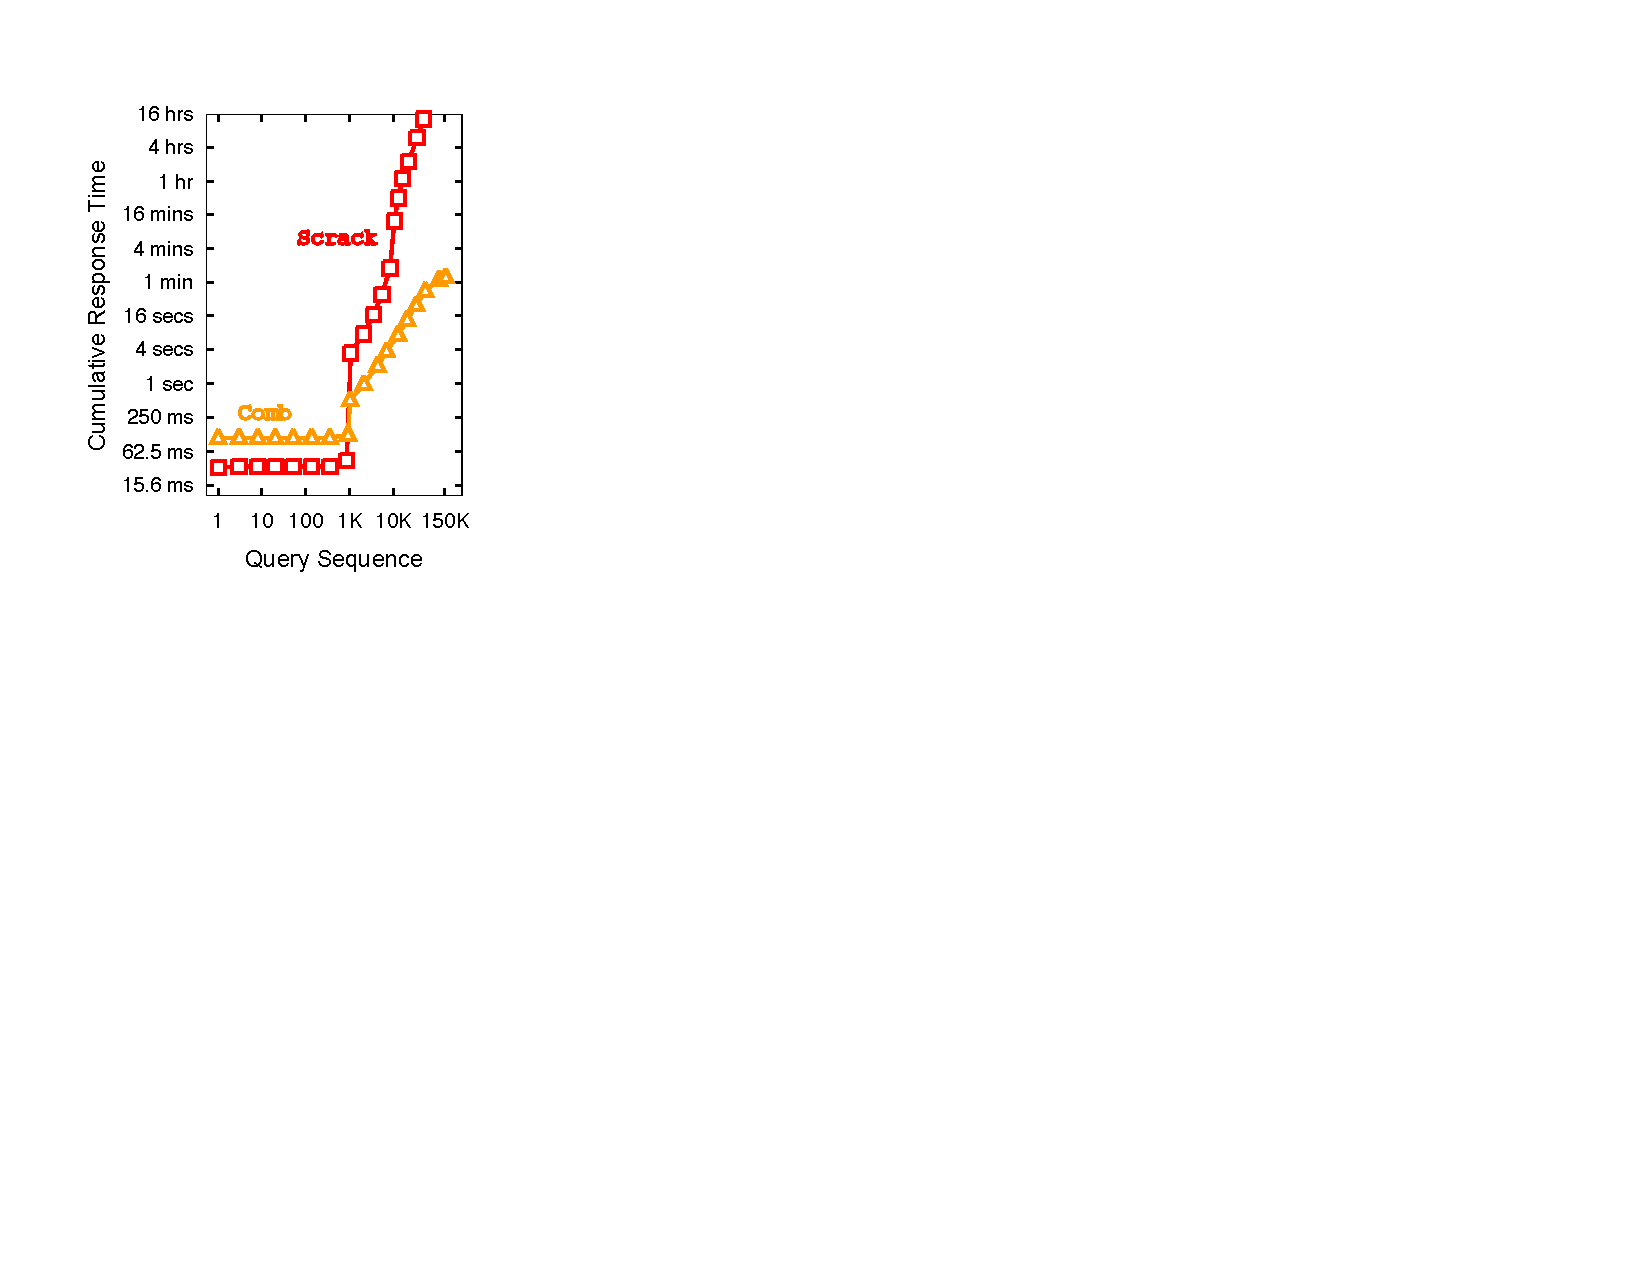
\includegraphics[width=.7\columnwidth]{graphs/fig_skyserver.pdf}%
\vspace{-1em}
\caption{SkyServer workload.}
\vspace{-1em}
\label{F:Skyserver}
}
\hfill
\hspace{-1.5em}%
\Fig[b]{.5\columnwidth}{%
\hspace{-.5em}%
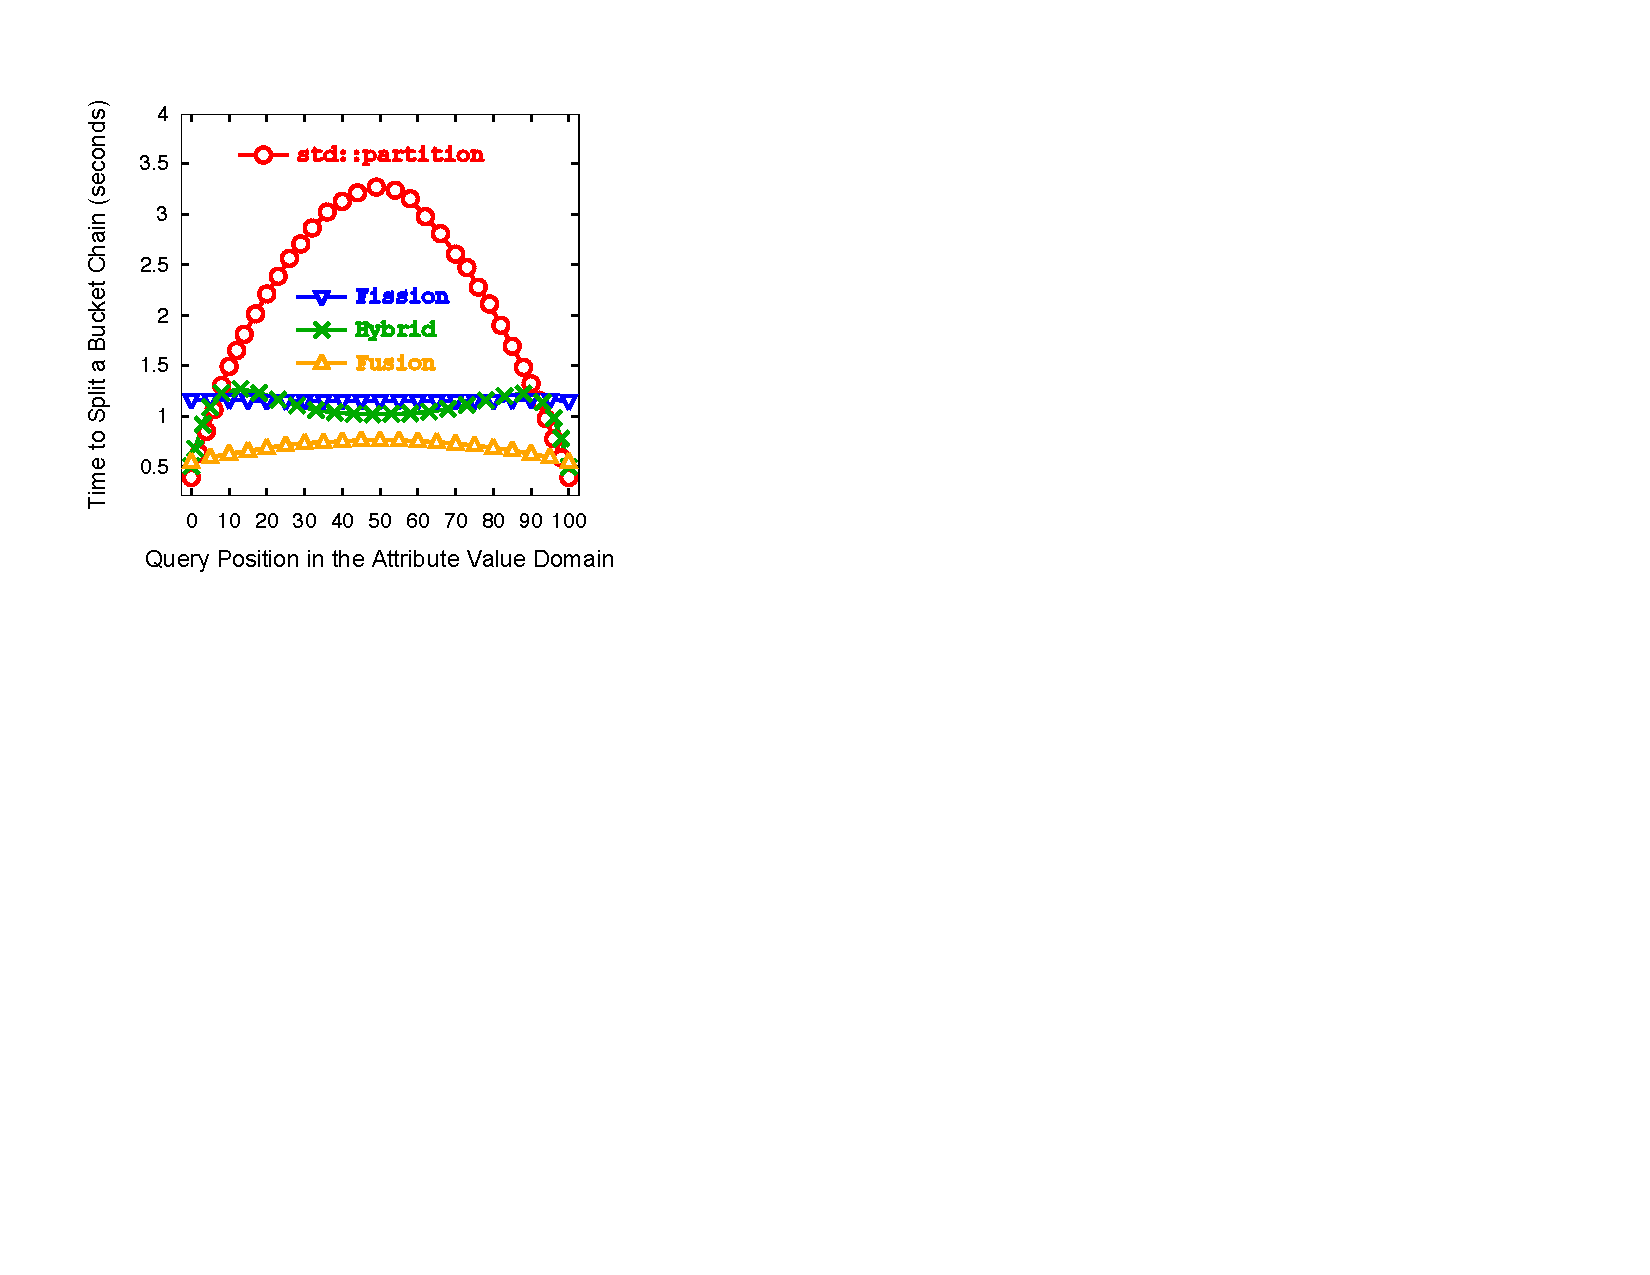
\includegraphics[width=1.055\columnwidth]{graphs/fusion.pdf}%
\vspace{-1em}
\caption{Bucket splitting.}
\vspace{-1em}
\label{F:fussion}
}
\end{figure*}

\section{Experimental Analysis}
\label{sec:experiments}

In this section, we present a detailed experimental analysis 
of Comb against state of the art adaptive indexing approaches using
both synthetic and real data sets. 
We compare Comb against original database cracking as well as against the latest 
evolutions of adaptive indexing namely stochastic database cracking \cite{StochasticCracking}, adaptive merging \cite{GK10b} 
and hybrid adaptive indexing \cite{AdaptiveIndexing}.
In addition, we compare Comb against the full indexing approach of fully sorting a column
as well as an in-memory B-tree index.
We demonstrate that Comb brings significant benefits outperforming these approaches
often by several orders of magnitude in long string of queries and updates. 


\newpage

\textbf{Resilient Adaptive Indexing.}
In our first experiment, we test Comb against original cracking in:
(i) a static many-queries scenario; and (ii) a scenario where many queries are interleaved by many updates.
The set up is the same as in the experiments of Section \ref{sec:problem}. 
The data consists of $10^8$ tuples of unique integers in $[0,2^{31})$.
The query workload is random; the ranges requested have a fixed selectivity of 1\% per query
but the actual bounds requested are random.
In the case of updates, 10 random inserts and 10 random deletes arrive every 10 read queries.

Figure \ref{F:BasicPerQueryComb} shows the results. 
In both the read only and in the updates scenario, Comb brings a significant advantage
and successfully handles the non-resilience problem of existing adaptive indexing. 
In the read only scenario in Figure \ref{F:BasicPerQueryComb}(a), 
Comb handles one billion queries in roughly fifteen minutes, while original database cracking
needs more than one hour. For the read scenario we also compare against the full indexing approach of sorting the 
column a priori. Comb is two times faster than full indexing in terms of total costs.
By carefully splitting the column in small pieces, and by keeping the buckets 
well balanced as well as 
by continuously refining the indexing information inside buckets, while adapting to the workload, Comb manages to be 
both lightweight and resilient in the long term.
Figure \ref{F:BasicPerQueryComb}(b) depicts the same results as Figure \ref{F:BasicPerQueryComb}(a) using 
logarithmic scales to more easily observe the early part of the query sequence.
Comb maintains the lightweight character of database cracking being ten times faster than the full indexing approach,
allowing for quick adaptation to the workload.
In addition, Comb starts materializing a benefit over cracking very early in the query sequence 
and in the end it is also roughly two times faster than the full indexing approach.

Figure \ref{F:BasicPerQueryComb}(c) depicts the update scenario; Comb manages to handle one billion queries in less than
one hour, while at the same time frame cracking only manages to answer 1000 times less queries, i.e., less than 1 million. 
Here, we do not include results with the full indexing approach as updating
a fully sorted column so often (every ten queries in this experiment), 
while still maintaining the dense structure of columns is prohibitively expensive.

Overall, Comb maintains both the lightweight and the adaptive character of cracking, while
bringing the resilience property, allowing to handle long strings of exploratory workloads
of continuous queries and updates.



\textbf{Comb on Real Workloads.}
For our next experiment, we demonstrate the benefits of Comb on
the SkyServer workload \cite{SkyServer}. SkyServer contains data from the astronomy domain 
and provides public database access to individual users and institutions.
We used an instance of the 4 Terabyte SkyServer data set and used $16*10^4$ queries from the query logs.
To focus on the adaptive indexing effect, i.e., within the select operator,
we filtered the selection predicates from queries.
Figure \ref{F:Skyserver} depicts the results for a sequence 
of queries using the ``right ascension" attribute of the ``Photoobjall" table.
The queries study a specific area of the sky
before moving on to a different area.
The Photoobjall table contains more than 500 million tuples, and it is one of the most commonly used ones in SkyServer. 
Data arrive continuously;
initially, only 10 million tuples are inserted. Then, every $10^3$ queries, 10 million more tuples arrive, reaching a total
of 500 million tuples by Query $5*10^4$; then another $10^4$ read only queries arrive.

Figure \ref{F:Skyserver} shows the results of comparing Comb against the state of the art 
stochastic cracking approach which was shown to be robust and more effective than plain cracking in \cite{StochasticCracking}. 
As soon as the update sequence begins, Comb materializes a significant benefit by being able to contain the update costs locally within its buckets with a small amount of data movements, 
while still being able to answer queries adaptively and efficiently.
In the end, Comb answers all queries in 1 minute, while stochastic cracking needs more than 16 hours.


\begin{figure*}[t]
\hspace{-1em}%
\Fig[b]{.95\columnwidth}{%
\hspace{1em}%
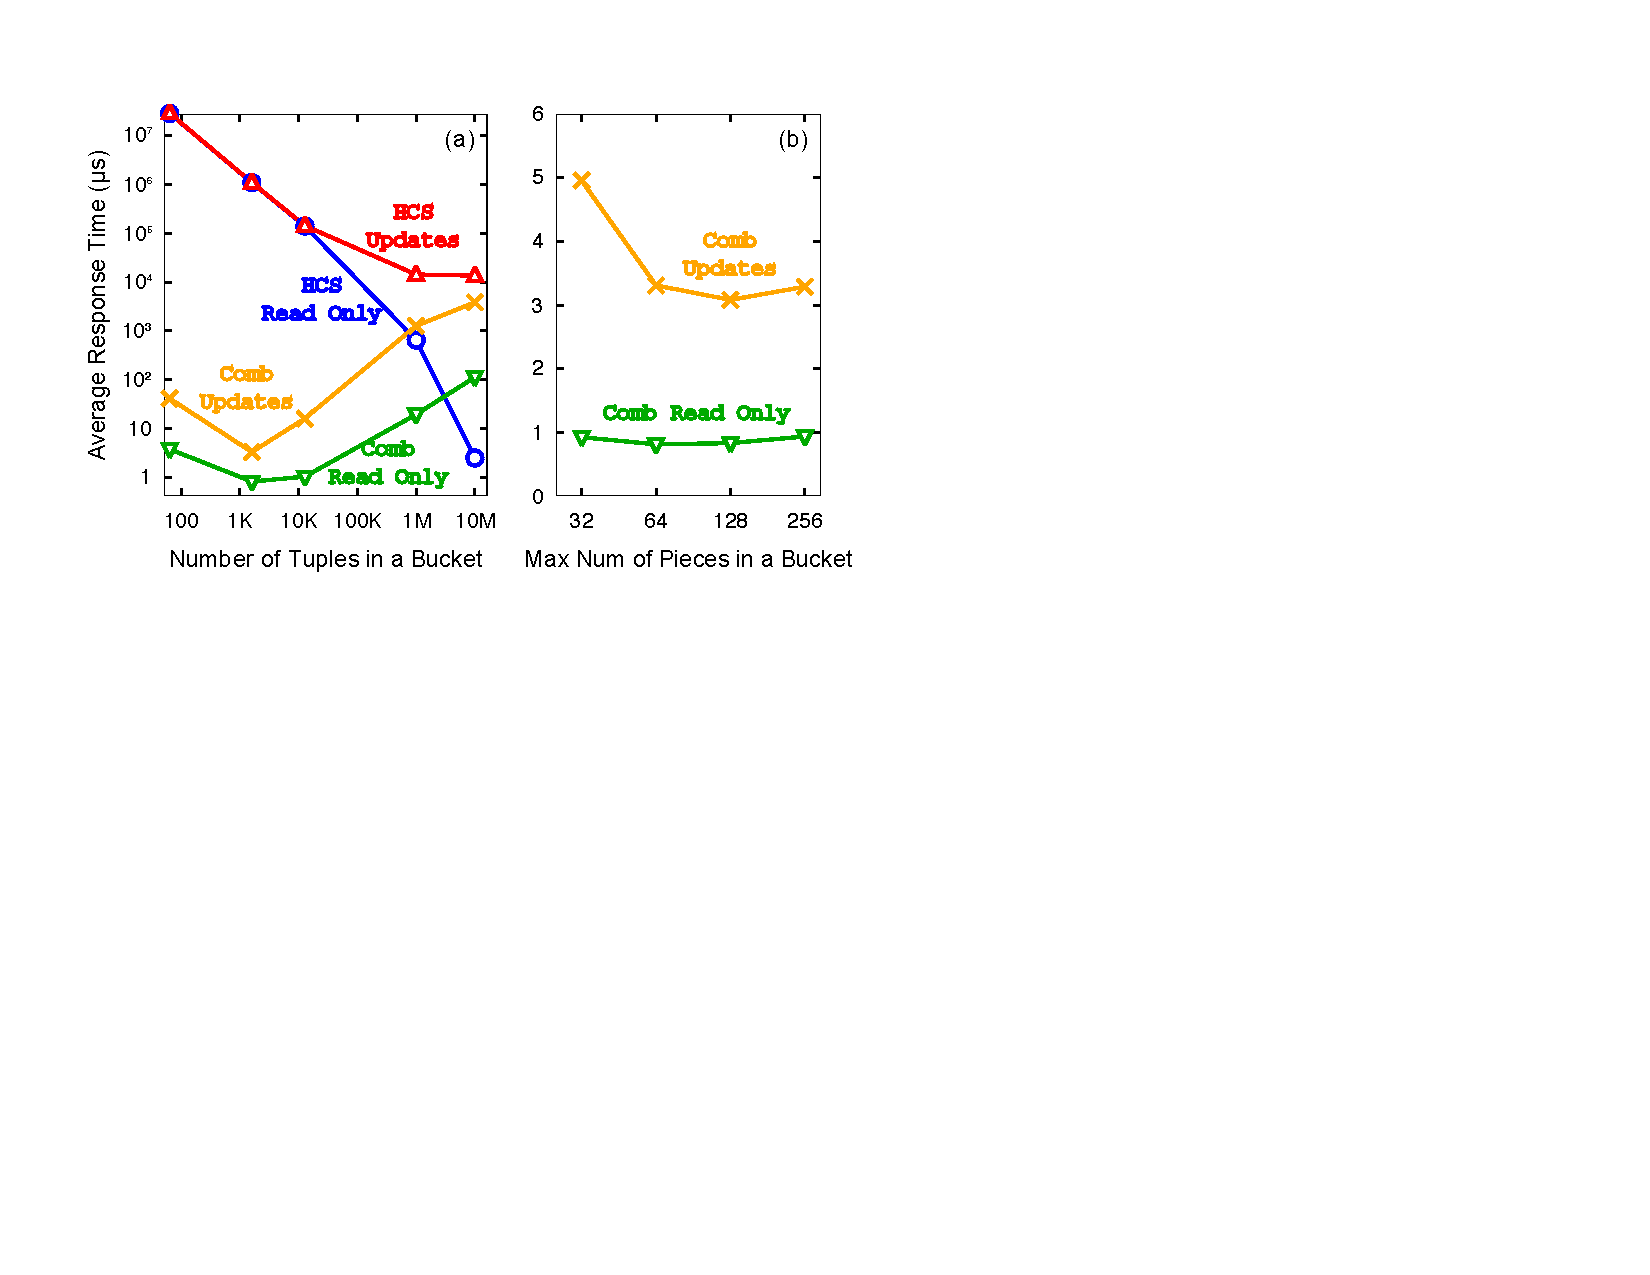
\includegraphics[width=.82\columnwidth]{graphs/hcs_comb.pdf}%
\vspace{-1em}
\caption{Varying bucket size and partitioning depth.}
\vspace{-1em}
\label{F:VaryBucketsPieces}
}
\hfill
\Fig[b]{.65\columnwidth}{%
\hspace{-3.7em}%
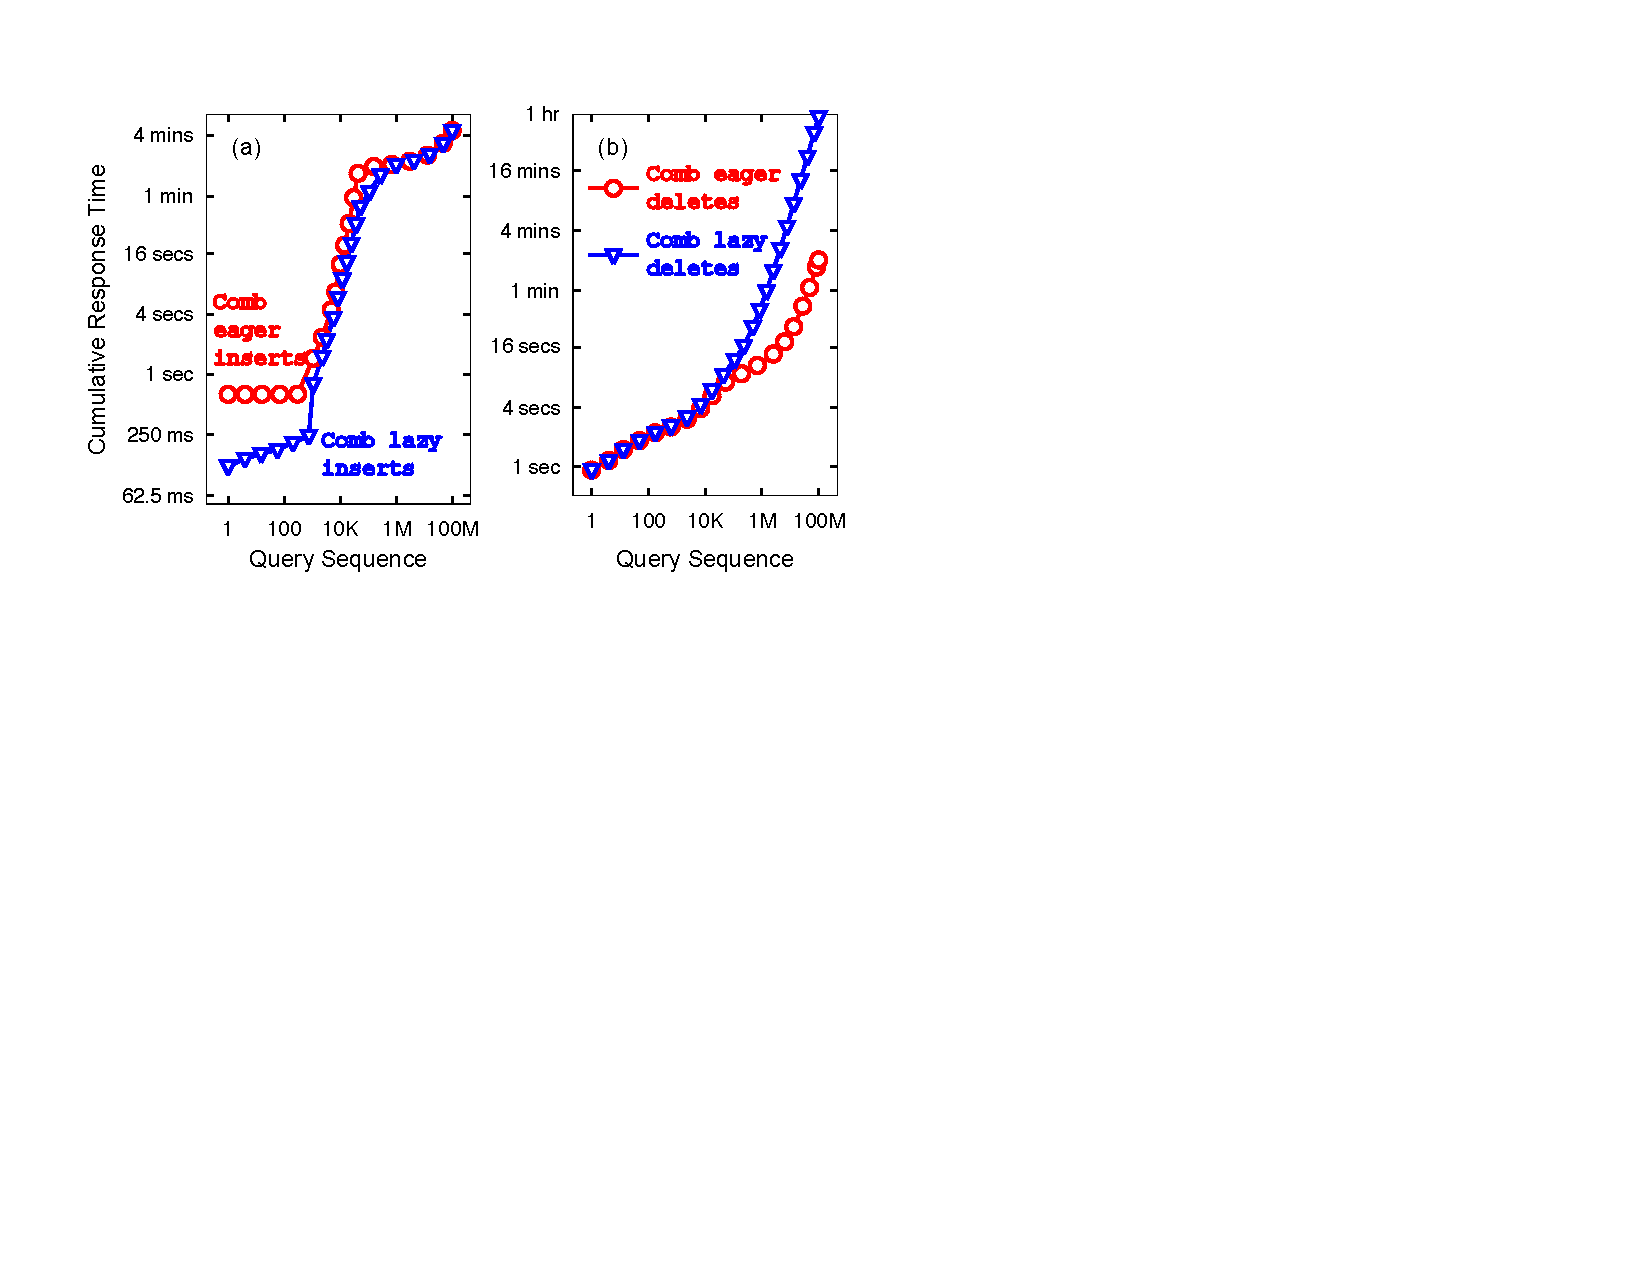
\includegraphics[width=1.2\columnwidth]{graphs/eager_lazy.pdf}%
\vspace{-1em}
\caption{Lazy V.s eager deletes/inserts.}
\vspace{-1em}
\label{F:LazyEager}
}
\hfill
\Fig[b]{.45\columnwidth}{%
\hspace{-.7em}%
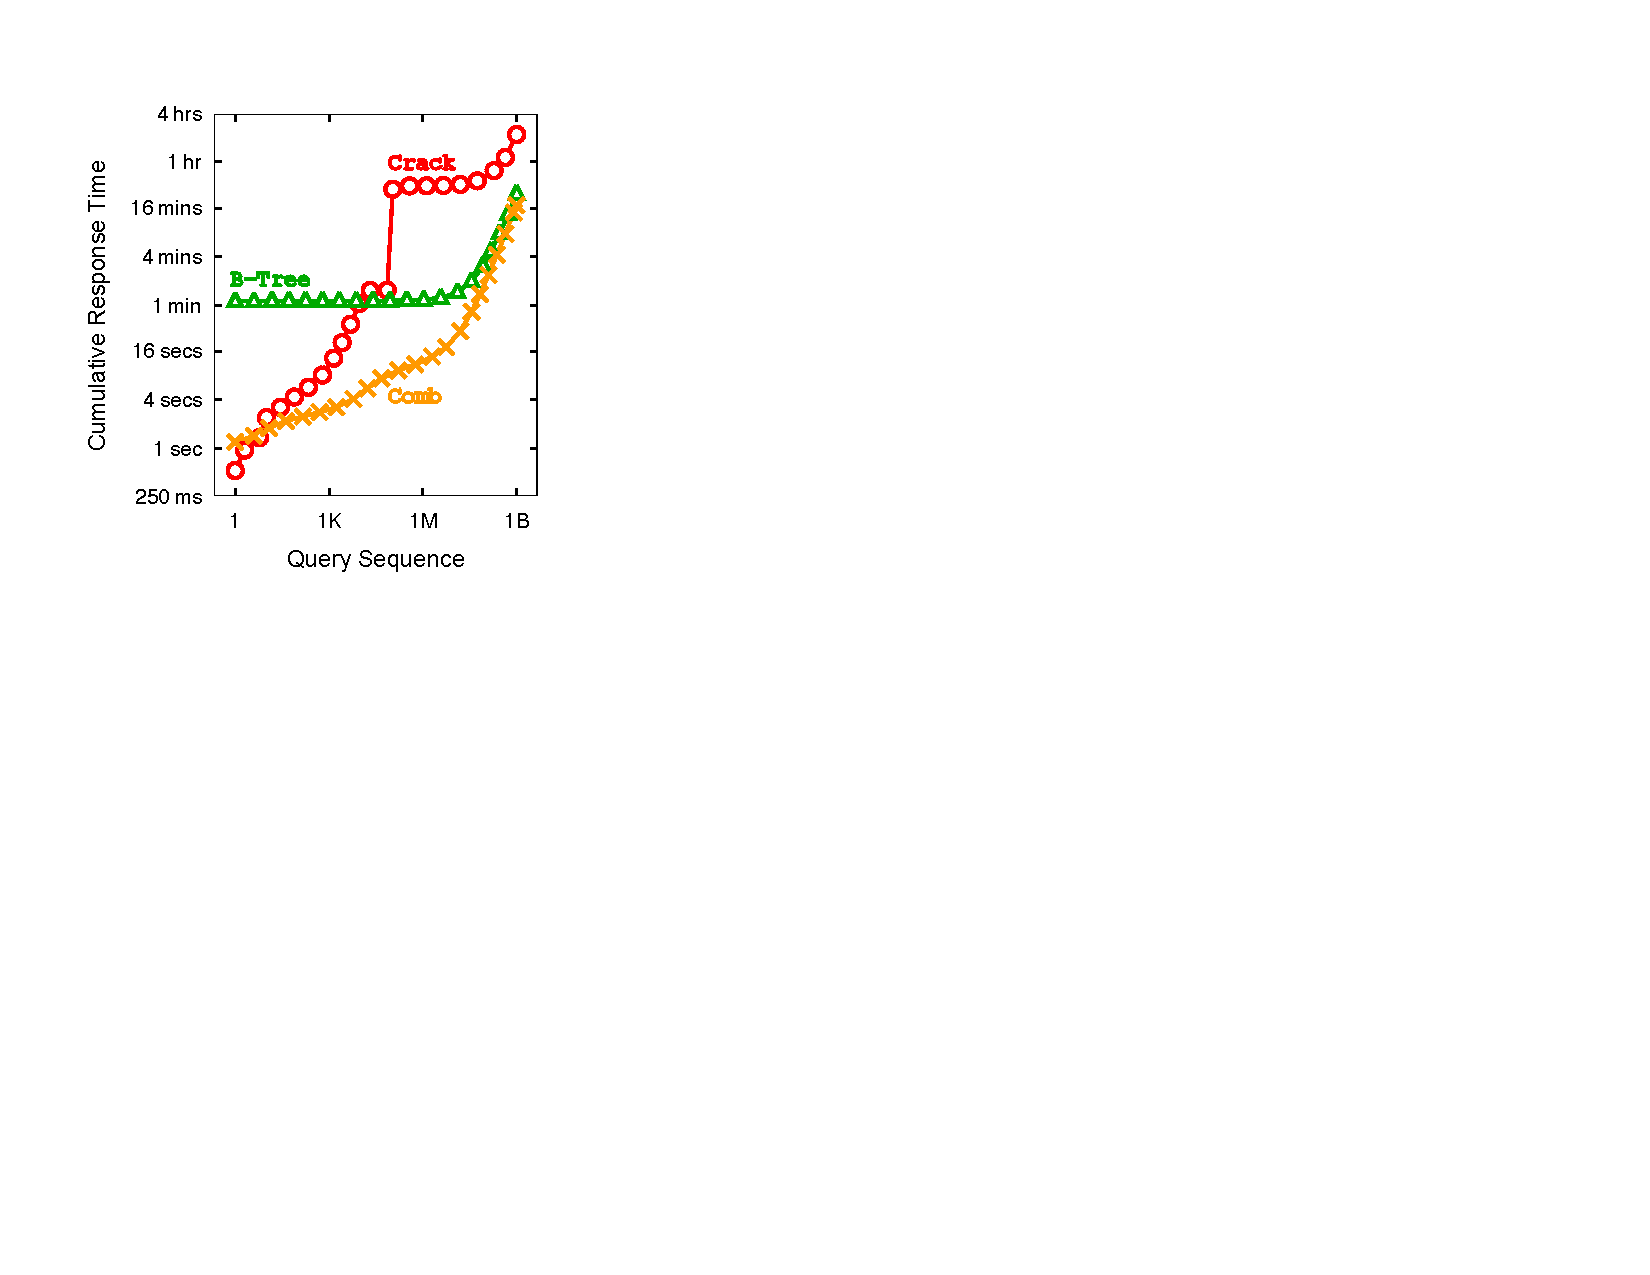
\includegraphics[width=1.06\columnwidth]{graphs/btree.pdf}%
\vspace{-1em}
\caption{Against B-tree.}
\vspace{-1em}
\label{F:Btree}
}
\end{figure*}


\textbf{Efficient Bucket Splitting.}
Splitting buckets adaptively during query processing is one of the most essential parts and cost components in Comb.
In this experiment, we demonstrate that expanding a standard partitioning algorithm is far from the optimal choice for splitting 
Comb buckets.
Figure \ref{F:fussion} demonstrates this effect. 
It shows the cost to split a chain of buckets in a Comb index. 
The chain consists of 512*256 buckets and each bucket contains 4*1024 tuples.
The $y$-axis depicts the cost to split all buckets in the chain, while varying the value of the pivot used for the splitting.
At the edges of the value domain, the pivot chosen splits a buckets in one small and one big piece, while in the 
middle of the value domain it splits the bucket in roughly two equal pieces.
Figure \ref{F:fussion} shows that when the pivot is chosen such that it splits buckets in half, the 
performance of the standard partitioning algorithm is quite poor compared to when a pivot is chosen 
at the edges of the domain. In the case of bucket splitting in Comb, we are especially interested in splitting buckets
in half such as  splitting can be effective and such that a query does less work (queries recursively split
bucket chains until they fall within a single bucket).

The reason for the poorer performance of the standard partitioning algorithm is that creating two 
equal partitions causes a significant number of branch mispredictions.
That is because the branches will fail half of the times not making it easy to predict.
Figure \ref{F:fussion} shows that our more lean chain splitting algorithm, Fission, does significantly better
by avoiding branches completely. 
Only at the very edges of the domain, standard partitioning outperforms the Fission alternative; 
then, there is no misprediction problem as all or or most branches take the same route.
Using an initial sampling phase, we are able to create a hybrid of the two approaches
where depending on the value range and the pivot we may choose the proper algorithm.
Figure \ref{F:fussion} shows that the hybrid version manages to keep the good properties of both standard partitioning and Fission.

Finally, Figure \ref{F:fussion} also depicts the behavior of the Fusion algorithm.
Fusion outperforms all other algorithms across the whole value domain.
Its strength comes from the fact that it combines the best properties from the previous variations.
It works without any branches for its core operations (as the Fission algorithm), 
while at the same time it minimizes data movements 
by doing a two pass process where it can first figure out which tuple should go where
and only then it starts moving tuples to their new location.   

 

\textbf{Effect of Bucket Size.}
Buckets are the fundamental block of Comb. 
By splitting the tuples across several buckets, Comb manages to 
handle updates and read accesses at a local per bucket level, improving 
data access patterns and minimizing data movements.
In this experiment, we study how the size of buckets may affect the performance of Comb.
As in our first experiment, the data consists of $10^8$ tuples of unique integers and queries
are chosen randomly and with a small selectivity 0.0001\%
(other selectivity factors are discussed later on). 
In the case of updates, 10 random inserts and 10 random deletes arrive every 10 queries.

Figure \ref{F:VaryBucketsPieces}(a) shows the results for both a read only scenario as well as for
a scenario where queries interleave with updates.
In both cases, a bucket size in the order of 1000-2000 tuples (in the case of 4 byte integers)
provides the best overall performance. This is a size where a bucket comfortably fits in L1 Cache.
A smaller size creates auxiliary administrative costs without bringing any more access benefits, while
a bigger size reduces administrative overheads but increases access and update costs.

Figure \ref{F:VaryBucketsPieces}(a) also depicts the performance of the state of the art hybrid adaptive 
algorithm HCS (hybrid crack-sort) which similarly to Comb also uses several buckets to store
tuples as opposed to a single column. Comb materializes a significant benefit especially when it comes 
to updates. HCS uses buckets which have overlapping value ranges and needs to physically move/merge data
to a second collection of buckets as queries arrive. On the contrary, Comb performs most of its 
index refinement actions in-place and continuously maintains buckets on non-overlapping value ranges
for the hot workload set. 
We also performed this experiment using adaptive merging (HSS \cite{AdaptiveIndexing}) which
resulted in similar performance to HCS; the only difference is that HCS is more lightweight
early in the query sequence. In the long run, performance degrades in the same way for both HCS and HSS. 



\textbf{Effect of Partitioning Depth.}
In order to reduce the excess administration and update costs, Comb puts a threshold on how deeply we can 
crack a given bucket, i.e., how many pieces we can create per bucket.
Figure \ref{F:VaryBucketsPieces}(b) shows the results of an experiment which studies the effect of 
how small or big this piece threshold should be.
The set-up is the same as in the previous experiment.
Given the small size of the bucket (set at default size of 1600 tuples) 
the number of pieces created do not significantly affect 
read only queries. In the case of updates though, there is a sweet point between 64 and 256 pieces
where both update and read costs are well balanced. The more pieces, the easier it is to locate 
a given range of tuples during a read query. On the other hand, more pieces force significant data movements
during updates. 
Comb uses 128 pieces per bucket as a default setting. 

\textbf{Eager Vs. Lazy Inserts.}
The default behavior of Comb is to chain buckets and adaptively split buckets 
during query processing and only for the ranges queried. 
This allows for an overall more lightweight behavior and an easy absorption of insertions.
In this experiment, we demonstrate the effect of a more eager strategy -- it
immediately splits buckets to place new tuples and balances the whole Comb structure during inserts.
The set-up is the same as in the previous experiment.
Figure \ref{F:LazyEager}(a) shows that overall the performance of the two approaches is rather similar in the long
run, while early in the query and update sequence the more lazy strategy allows for a more lightweight
and quick adaptation to the workload which is one of the main motivations of adaptive indexing.

\textbf{Eager Vs. Lazy Deletes.}
As we discussed in Section \ref{sec:cracke}, Comb uses a default strategy where deletes are eagerly merged
in buckets. This choice is to guarantee robustness.
Our next experiment demonstrates this behavior. 
Using a similar set-up as the previous experiments we fire a long  sequence of queries and deletes;
every 10 read queries we get 10 deletes.
Figure \ref{F:LazyEager}(b) compares the behavior of eager versus lazy deletes in Comb. 
As the sequence evolves eager deletes materialize a significant benefit;
Comb can answer 100M queries in less than 4 minutes, while with lazy deletes it needs more than 1 hour.
The main disadvantage of the lazy deletes comes from the fact that we need to check all buckets
that qualify for a range query and merge the qualifying pending deletes. This puts a significant overhead at query time. 

In the case of insertions, where Comb does use lazy inserts as a default strategy, Comb does not have to do any significant
actions during query processing. That is because inserts are placed already in the proper bucket;
they are simply out of place in terms of their local organization within the bucket.
So in a range query such as the one showed in Figure \ref{F:rangequery}, Comb only needs
to do merging actions for pending inserts for the two bound buckets at the edges of the qualifying value range. 
All buckets in between qualify but no action needs to be taken as we know that all data qualifies anyway.






\textbf{Comparison with B-tree.}
In our next experiment, we compare against a modern in-memory B-tree\footnote{\small We use the STX B+ Tree v0.8.6 (http://idlebox.net/2007/stx-btree/).} 
in a scenario where updates happen in big batches but more rarely than in previous experiments.
Using a column of $10^8$ tuples as before, this time we fire $10^6$ random inserts
just before Query 10 and another  $10^6$ random inserts just before Query $10^5$.
With original cracking, the inserts cause future queries to degrade in performance 
as they try to merge inserts in. The B-tree can handle the insertions in a graceful way
but it has a high initialization cost. 
Comb shows the same stability as the B-tree and the same lightweight adaptation as the
initial part of the cracking curve, combining the best of both worlds.  




\begin{figure}[t]
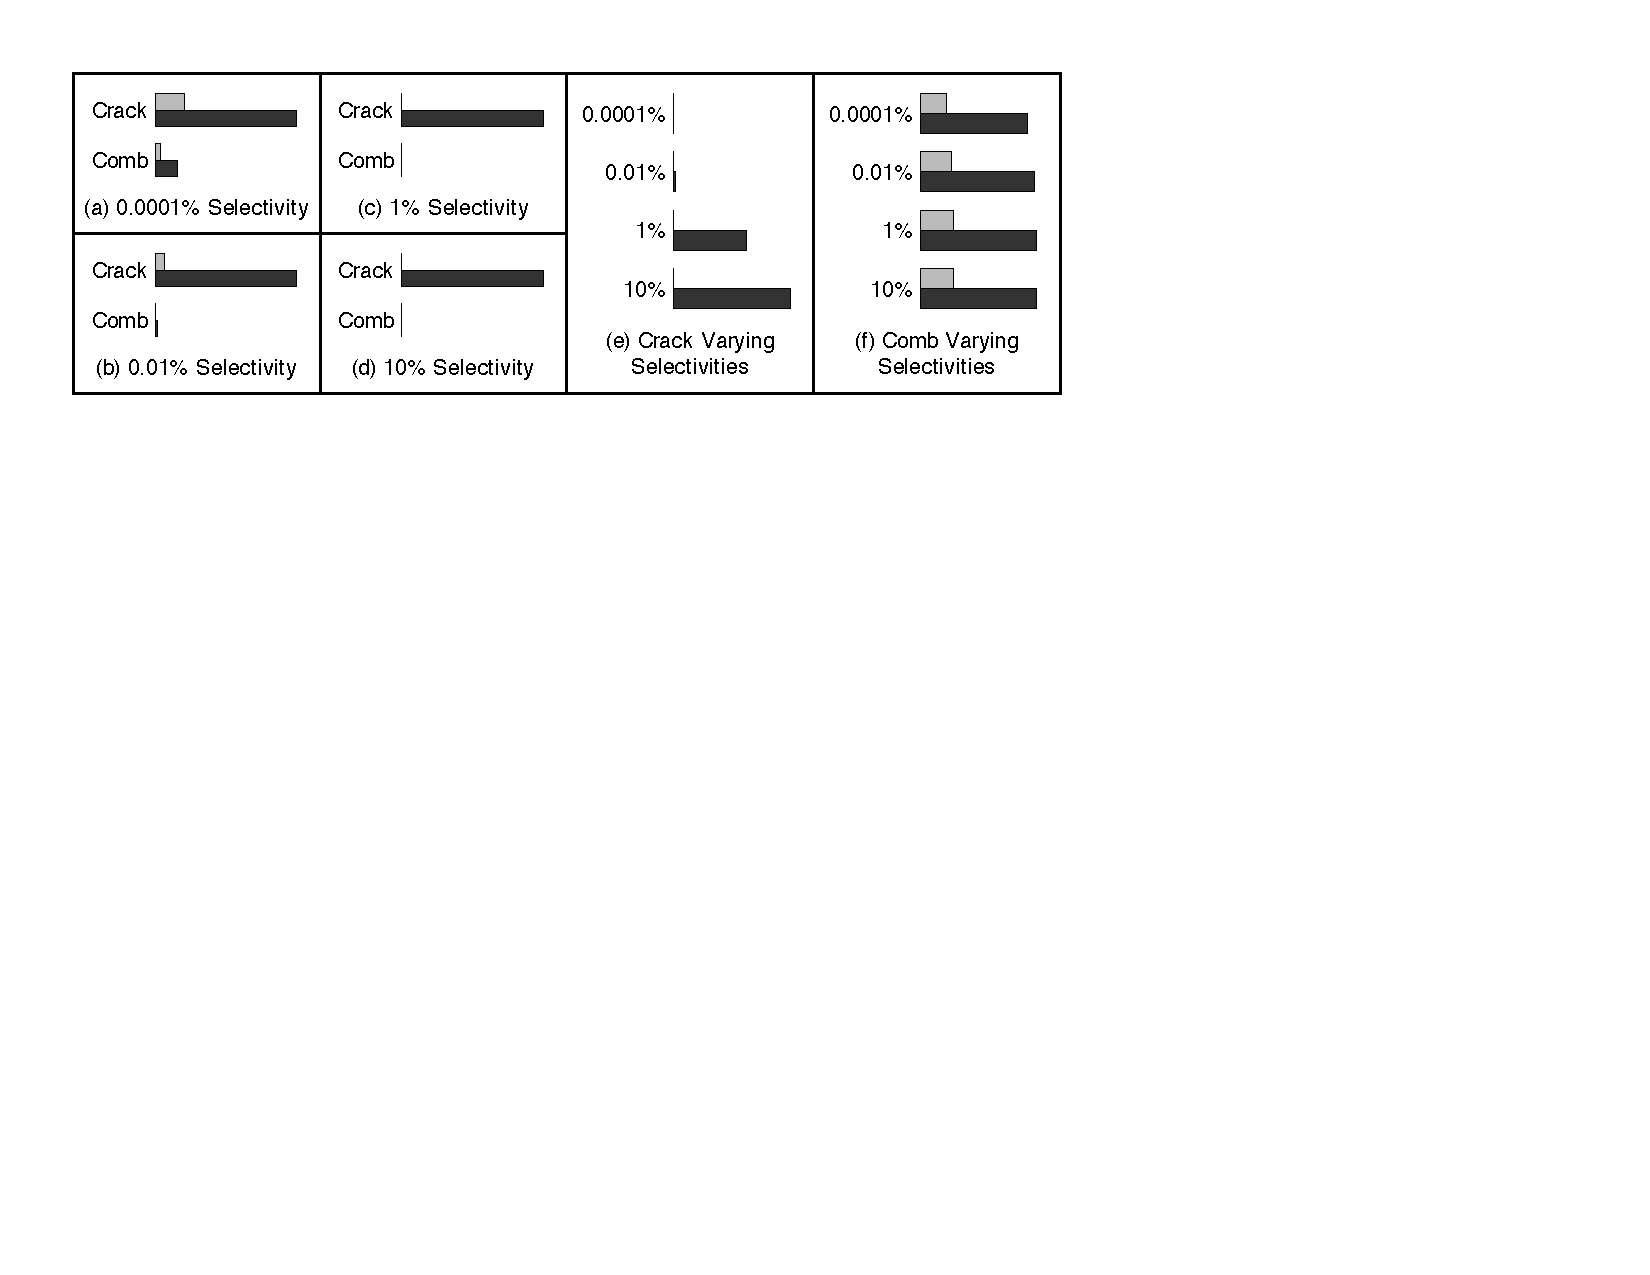
\includegraphics[width=\columnwidth]{graphs/selectivities.pdf}%
\vspace{-1em}%
\caption{Varying selectivity.}
\vspace{-2em}%
\label{F:Selectivity}
\end{figure}

\textbf{Varying Selectivity.}
In our next experiment, we demonstrate the effect of varying selectivity.
The set-up is the same as in our first experiment  with the difference that we vary the selectivity in queries.
Figure \ref{F:Selectivity} shows the results.
Figures \ref{F:Selectivity}(a)-(d) show the results for various selectivity factors.
In each box, the bars indicate normalized average query response time
with grey bars for read-only workloads and black bars when
updates interleave with queries.\footnote{
\small
We caution that normalization means that different boxes cannot be compared
as the normalization factor varies.
}
The result shows that Comb has a significant advantage across all selectivity factors.
Then, Figure \ref{F:Selectivity}(e) shows that as we vary selectivity database cracking shows a non-resilient performance
for the update workloads. What happens is that as we select bigger value ranges and thus more tuples, 
more pending updates need to be merged causing excessive update costs.
Comb on the other hand does not suffer. 
Figure \ref{F:Selectivity}(f) shows that the performance of 
Comb is stable across all selectivity factors providing a resilient and  reliable performance. 

\textbf{Optimizing Existing Adaptive Indexing.}
In our final experiment, we demonstrate that simple solutions to patch existing adaptive indexing
solutions cannot achieve the same performance as Comb which is designed from scratch for
long exploratory sequences of queries and updates.
Figure \ref{F:SimpleApproaches} shows the behavior of Comb against the 4 approaches described in Section \ref{sec:simple}.

Figures \ref{F:SimpleApproaches}(a), (b) and (c) compare Comb against the Crack-Scan, Crack-NoIndex and Crack-Sort approaches.
The experiment also varies the amount of tuples we allow inside a cracking piece in the cracker index before we choose to switch 
to the scan, sort or no-index strategy for each approach. 
As in the previous experiment, each box gives the normalized query response time
with grey bars for read-only performance
and black bars when updates interleave with queries.
Crack-Scan and Crack-NoIndex do manage to improve over plain cracking especially as the piece size threshold
becomes smaller (resulting in more pieces overall). Crack-Sort brings an extra overhead due to the expensive sorting step. 
In all cases, though, Comb manages to significantly outperform all approaches	being always 3-4 times faster than 
the second fastest approach.  


\begin{figure}[t]
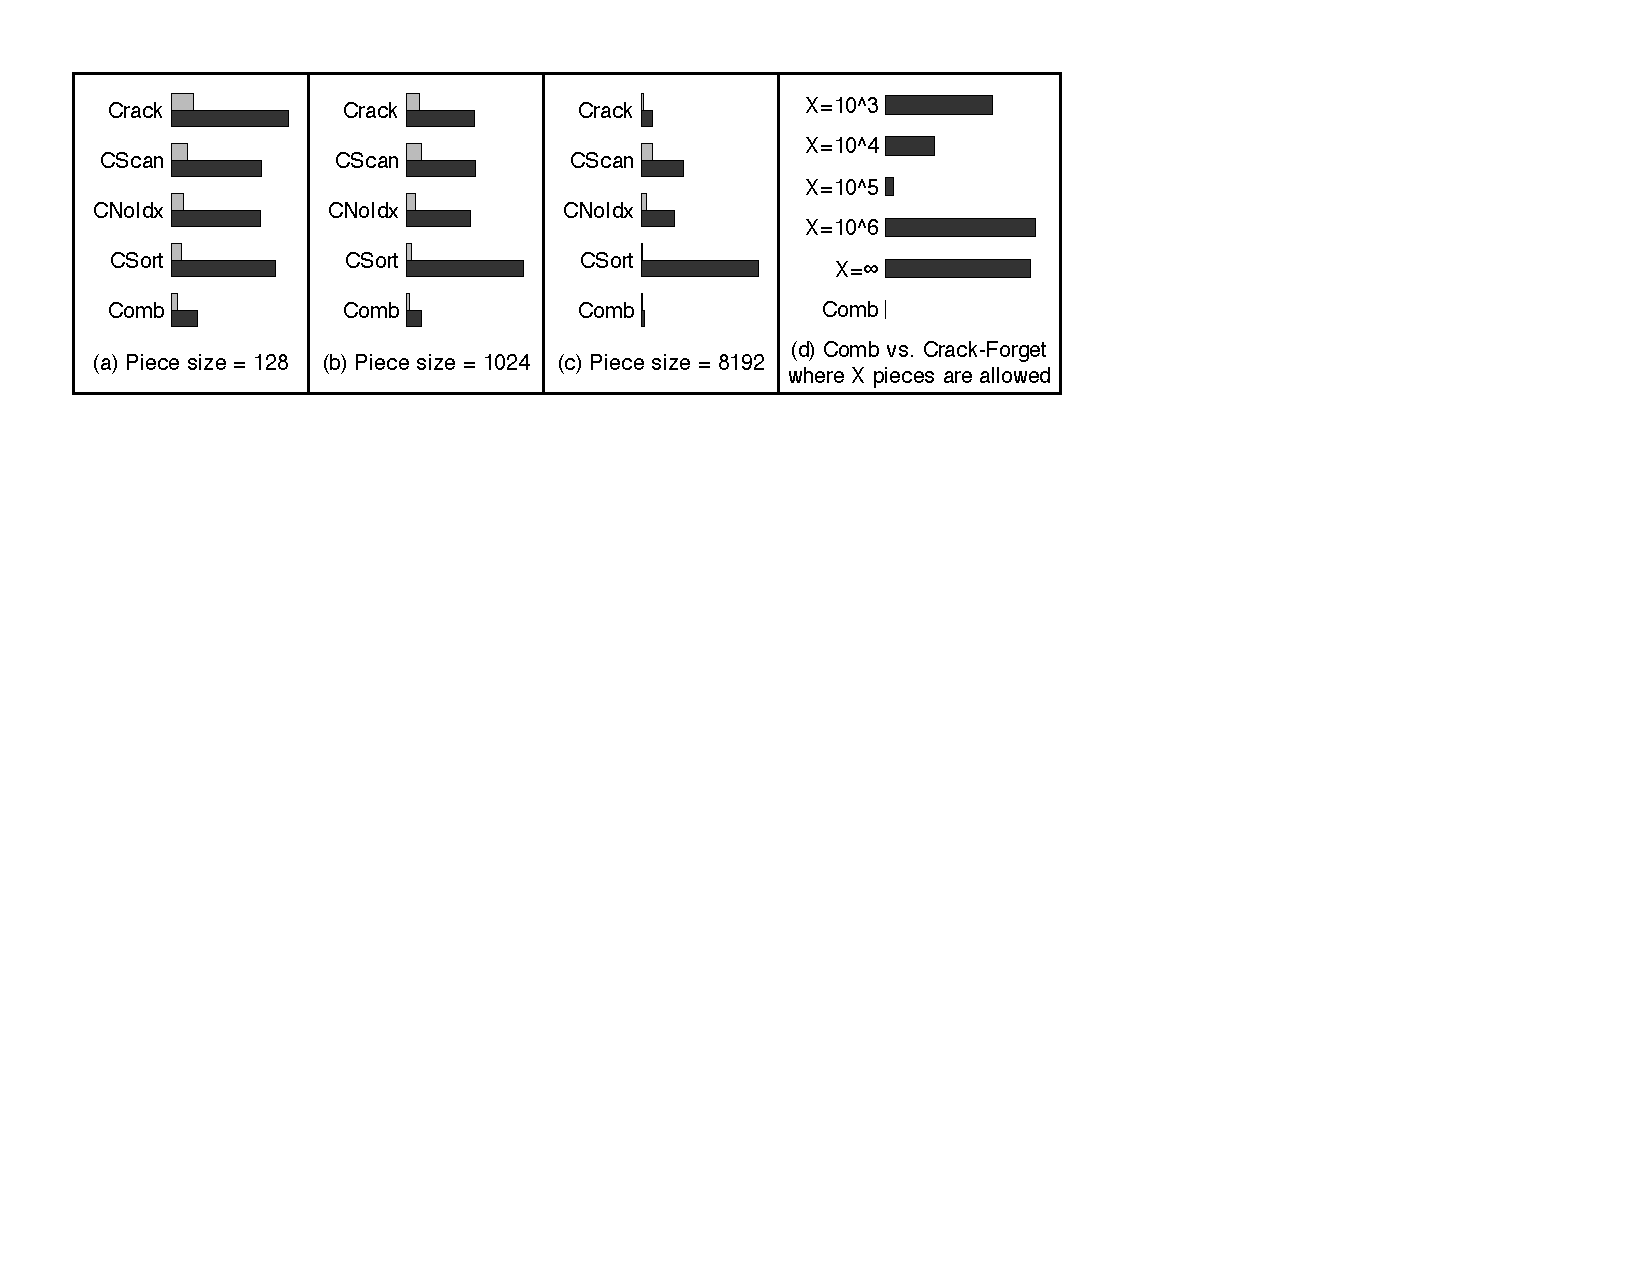
\includegraphics[width=\columnwidth]{graphs/fig_simple_w_crake.pdf}%
\vspace{-1em}%
\caption{Optimizing existing adaptive indexing.}
\vspace{-1em}%
\label{F:SimpleApproaches}
\end{figure}

Figure \ref{F:SimpleApproaches}(d) shows the performance of Comb against the Crack-Forget approach
which extends original database cracking with the ability to adaptively remove indexes
when it realizes that it needs to do expensive update actions.
It limits how many pieces it can have in the cracker index;
if the number of pieces is beyond this threshold, then  pieces which are about to be updated
are adaptively removed during query processing and thus the merging actions for updates become much more lightweight.
Figure \ref{F:SimpleApproaches}(d) shows the performance (normalized) while varying the piece threshold.
Even in the best case for Crack-Forget, Comb is 2 orders of magnitude faster.

Overall, Comb is able to outperform all patches in existing adaptive indexing approaches
and by being able to balance the costs across multiple buckets, while containing
administrative costs locally, it brings a significant performance advantage and is resilient.

 
